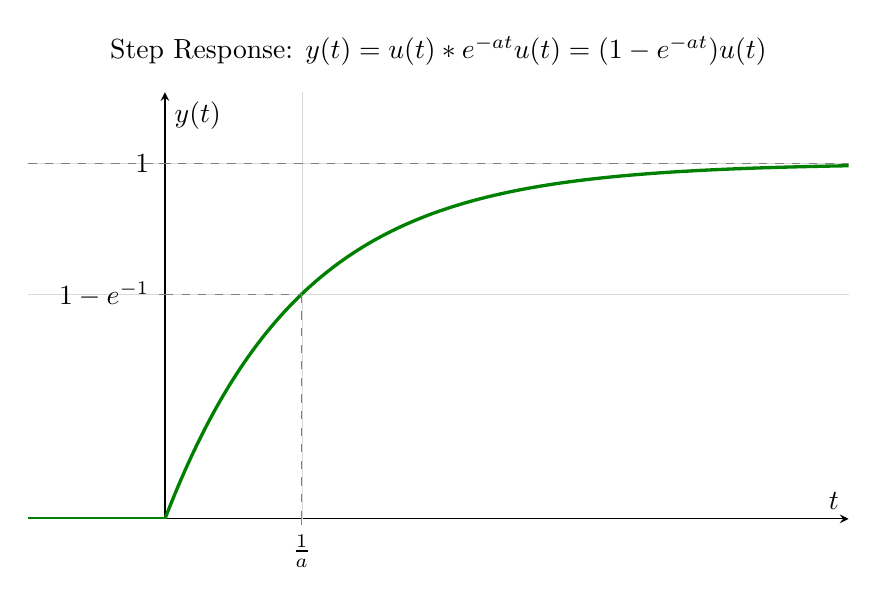
\begin{tikzpicture}
	\begin{axis}[
		width=12cm,
		height=7cm,
		title={Step Response: $y(t) = u(t) * e^{-at}u(t) = (1-e^{-at})u(t)$},
		xlabel={$t$},
		ylabel={$y(t)$},
		axis lines=middle,
		xmin=-1, xmax=5,
		ymin=0, ymax=1.2,
		xtick=\empty,
		ytick=\empty,
		extra x ticks={1},
		extra x tick labels={$\frac{1}{a}$},
		extra y ticks={0.632, 1},
		extra y tick labels={$1-e^{-1}$, $1$},
		grid=major,
		grid style={line width=.1pt, draw=gray!30},
		]
		
		% Plot the step response for a=1
		\addplot[green!50!black, very thick, domain=0:5, samples=200, no marks] {1 - exp(-x)};
		\draw[green!50!black, very thick] (axis cs:-1,0) -- (axis cs:0,0);
		
		% Plot the asymptote
		\addplot[dashed, gray, domain=-1:5] {1};
		
		% Add guidelines for the time constant
		\draw[dashed, gray] (axis cs:1,0) -- (axis cs:1, {1-exp(-1)});
		\draw[dashed, gray] (axis cs:0, {1-exp(-1)}) -- (axis cs:1, {1-exp(-1)});
		
	\end{axis}
\end{tikzpicture}